% Chapter Template

\chapter{Experimentos}

\label{Chapter5} % Change X to a consecutive number; for referencing this chapter elsewhere, use \ref{ChapterX}

En este capítulo se detallarán las pruebas realizadas, con el objetivo de validar la solución propuesta en este trabajo. Además se comprobarán las diferentes configuraciones desarrolladas y se evaluarán sus prestaciones con los costes temporales. Estos experimentos han permitido depurar el componente para poder ajustar y mejorar la funcionalidad del mismo durante el desarrollo.

%-----------------------------------
%	SECTION Validación experimental
%-----------------------------------
\section{Validación experimental}

El entorno de pruebas utilizado ha sido siempre un entorno real, trabajando con los datos en vivo proporcionados por OpenniServer que extrae la información directamente del sensor.

Se propone en esta sección validar el componente en las diferentes fases que lo componen: detección de puntos de interés, cálculo de emparejamientos y estimación de movimiento.

\subsection{Detección de puntos de interés}



\subsection{Cálculo de emparejamientos}


\subsubsection{Posición estática}
\subsubsection{Traslación}
\subsubsection{Rotación}


\subsection{Resolución 3D}

La resolución 3D o estimación de movimiento compone el último paso que completa una iteración del sistema, por lo que en esta etapa podremos ver el resultado final del movimiento entre varios fotogramas consecutivos.

Las pruebas mostrados a continuación son realizadas con un funcionamiento normal del componente y en un tiempo determinado. El objetivo de estos experimentos es comprobar el comportamiento del sistema para los diferentes tipos de traslaciones ($x$, $y$, y $z$) y rotaciones (\textit{pitch}, \textit{yaw}, \textit{roll}).

Para estas pruebas y las siguientes se hará uso del componente con el comportamiento automático activado, repitiendo así de manera autónoma cada ciclo de estimación 3D.

\subsubsection{Validación de la traslación}
\subsubsection{Validación de la Rotación}
\subsubsection{Validación de trayectorias complejas}

\subsection{Error estático}

El error estático muestra el ruido blanco que se esconde detrás de la resolución 3D en tiempo real. Como se va a poder observar en esta sección, el ruido estático es inevitable y no depende del algoritmo a utilizar. Sin embargo, en el siguiente capítulo, en el cual se propone posibles mejoras y líneas futuras, se verán métodos para poder elimnarlo en mayor o menor medida.

En las siguientes Figuras (\ref{fig:static1}, \ref{fig:static2}, \ref{fig:static3}) se puede ver un ejemplo de este error para diferentes configuraciones. Como se puede interpretar es un error que está presente en todos los casos.

\begin{figure}[th]
\centering
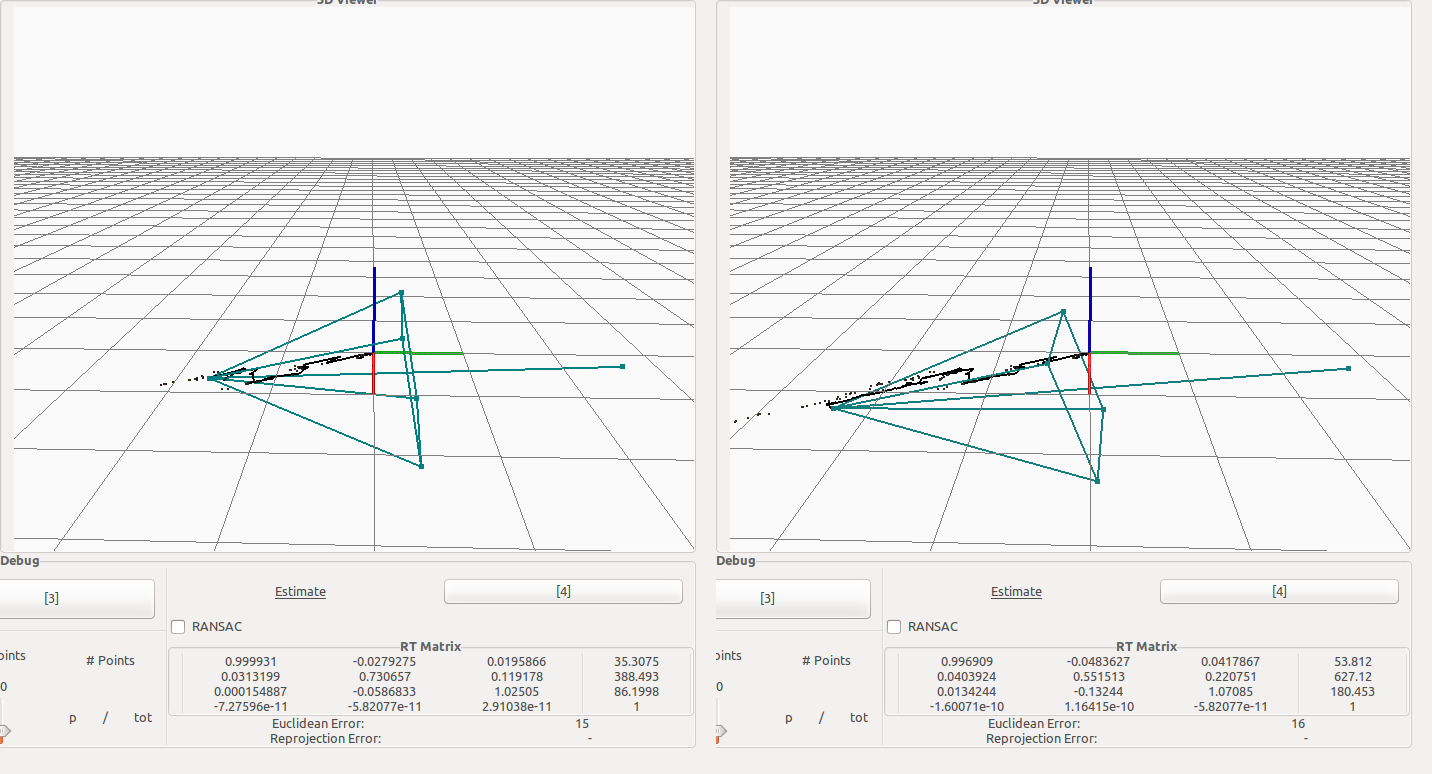
\includegraphics[scale=0.3]{Figures/tests/static-surf-flann_2.png}
\decoRule
\caption[Ruido estático, con SURF y FLANN]{Ruido estático después de 30 y 60 segundos, con SURF y FLANN.}
\label{fig:static1}
\end{figure}

\begin{figure}[th]
\centering
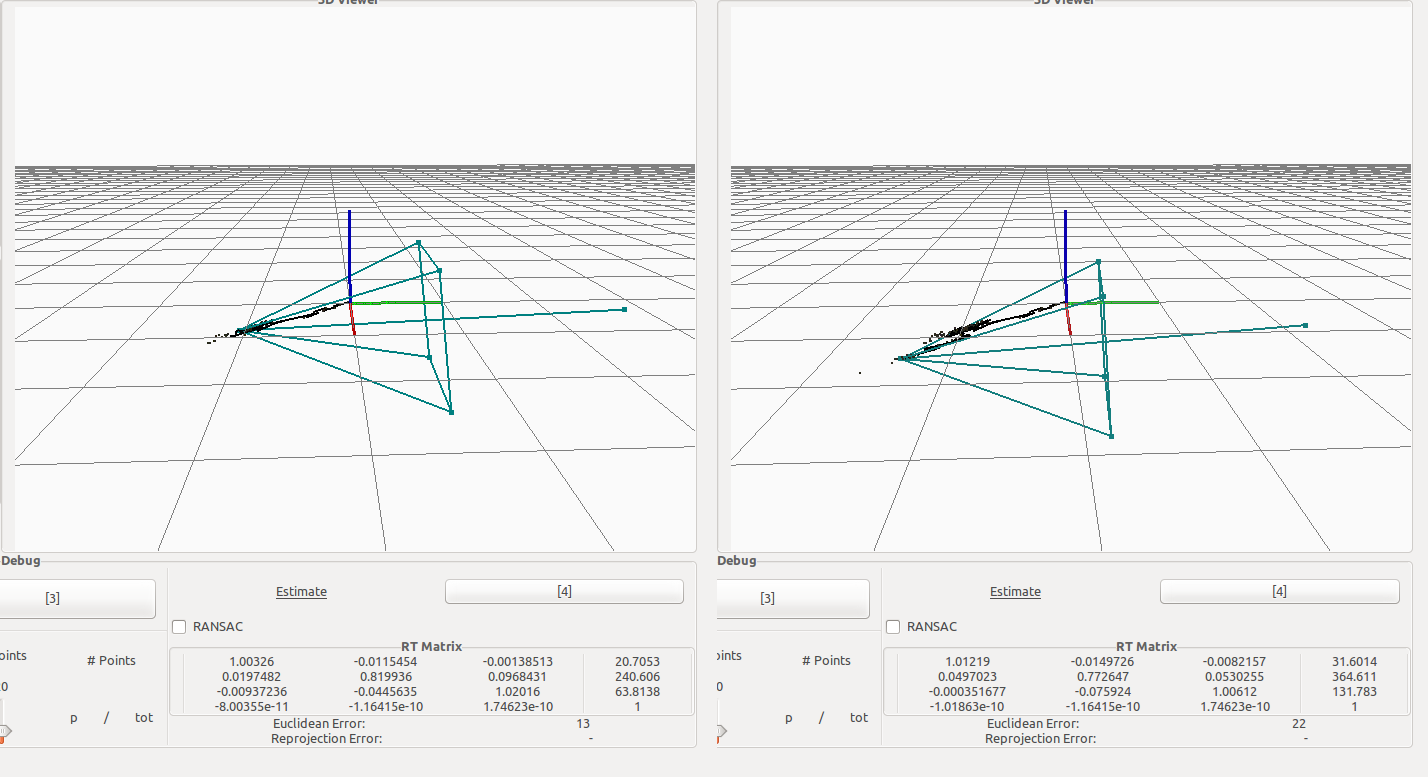
\includegraphics[scale=0.3]{Figures/tests/static-filter_2.png}
\decoRule
\caption[Ruido estático, con SIFT, Fuerza Bruta y filtros]{Ruido estático después de 30 y 60 segundos, con SIFT, Fuerza Bruta y filtros.}
\label{fig:static2}
\end{figure}

\begin{figure}[th]
\centering
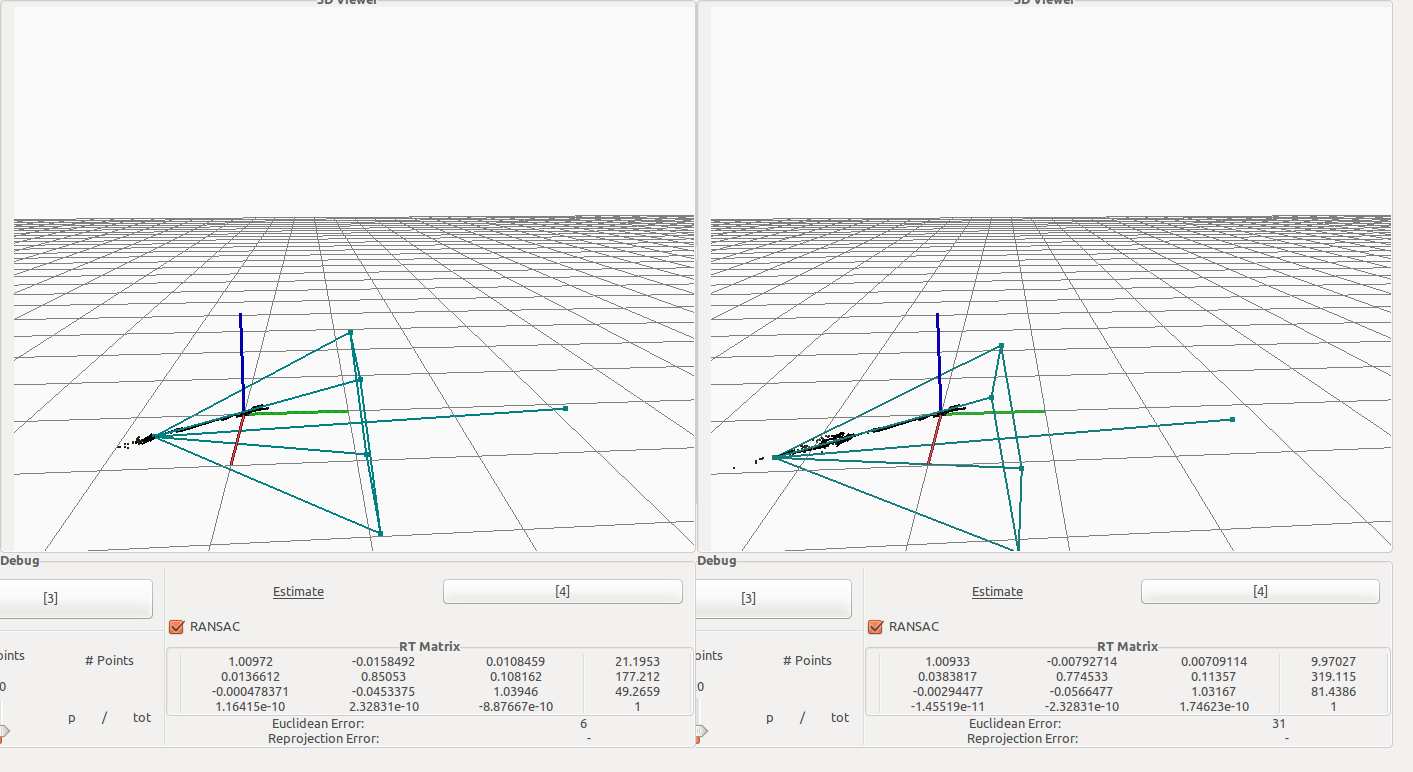
\includegraphics[scale=0.3]{Figures/tests/static-ransac_2.png}
\decoRule
\caption[Ruido estático, con SIFT, Fuerza Bruta y RANSAC]{Ruido estático después de 30 y 60 segundos, con SIFT, Fuerza Bruta y RANSAC.}
\label{fig:static3}
\end{figure}

Las pruebas realizadas han sido capturadas a los 30 y 60 segundos respectivamente y la configuración aplicada se encuentra en la descripción de cada Figura.

Si analizamos las matrices RT obtenidas se puede observar que el eje en que más avanza el ruido es el eje $y$, que es el perpendicular al plano imagen y el que se obtiene de la imagen de profundidad.


%-----------------------------------
%	SECTION Tiempos de procesado
%-----------------------------------
\section{Tiempos de procesado}